%przyklady uzyskiwanych efektow pracy aplikacji (wyniki eksperymentow)

\section{Aplikacja}
Na rysunkach \ref{fig:pusty} - \ref{fig:niewazkosc_stabilny} znajdują się przykłady uzyskiwanych efektów pracy aplikacji. Przetestowane zostały jej wszystkie założone funkcjonalności.

\begin{minipage}{0.5\textwidth}
\begin{figure}[H]
 \begin{center}
  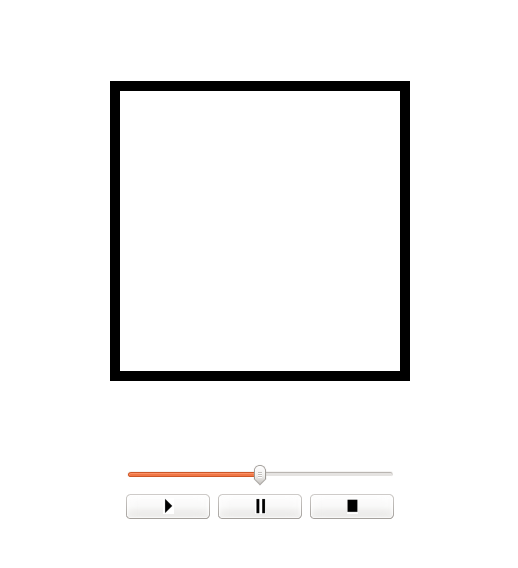
\includegraphics[width=\textwidth]{./rysunki/pusty}
 \end{center}
 \caption{Pusty zbiornik}
 \label{fig:pusty}
\end{figure}
\end{minipage}
~
\begin{minipage}{0.5\textwidth}
\begin{figure}[H]
 \begin{center}
  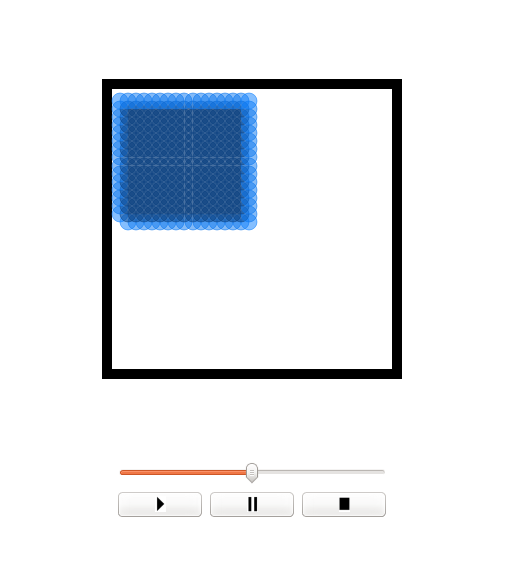
\includegraphics[width=\textwidth]{./rysunki/poczatek}
 \end{center}
 \caption{Wybrany stan początkowy}
 \label{fig:poczatek}
\end{figure}
\end{minipage}\\[0.1cm]

\begin{minipage}{0.5\textwidth}
\begin{figure}[H]
 \begin{center}
  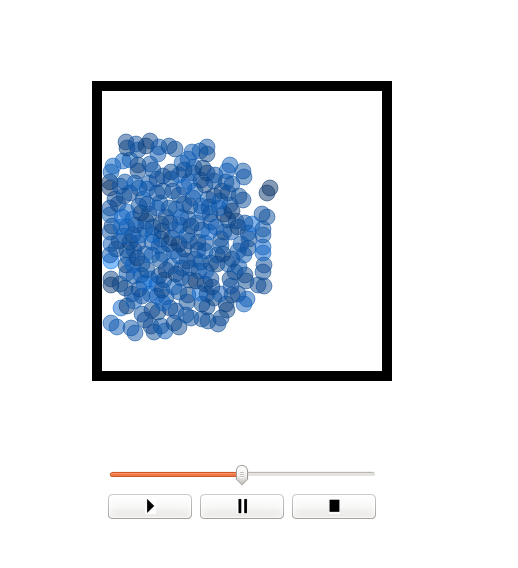
\includegraphics[width=\textwidth]{./rysunki/poczatek2}
 \end{center}
 \caption{Symulacja}
 \label{fig:poczatek2}
\end{figure}
\end{minipage}
~
\begin{minipage}{0.5\textwidth}
\begin{figure}[H]
 \begin{center}
  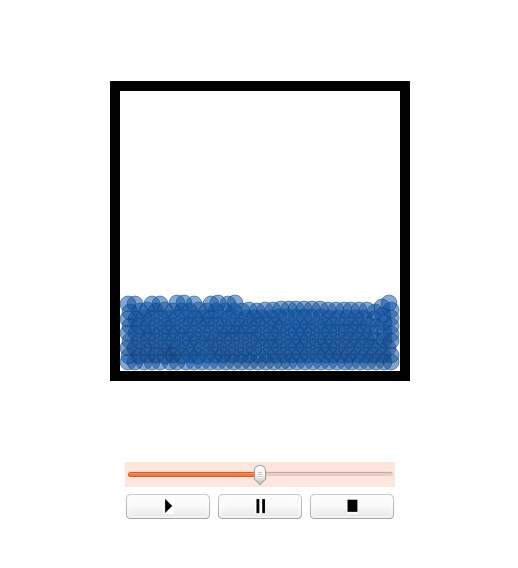
\includegraphics[width=\textwidth]{./rysunki/plasko_stabilny}
 \end{center}
 \caption{Ustabilizowana ciecz}
 \label{fig:plasko_stabilny}
\end{figure}
\end{minipage}\\[0.1cm]

\begin{minipage}{0.5\textwidth}
\begin{figure}[H]
 \begin{center}
  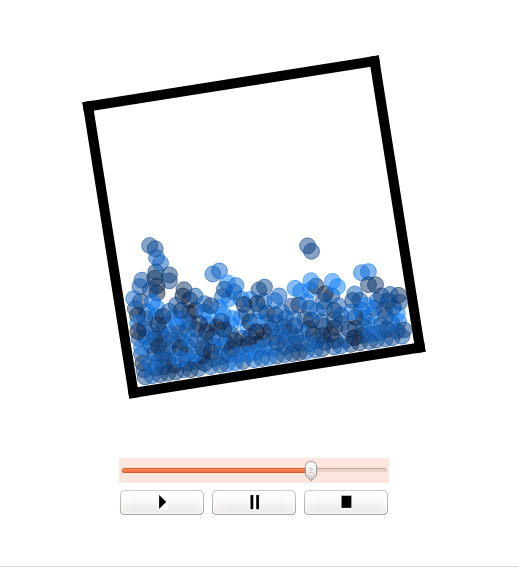
\includegraphics[width=\textwidth]{./rysunki/obrot_niestabilny}
 \end{center}
 \caption{Obracanie zbiornika}
 \label{fig:obrot_niestabilny}
\end{figure}
\end{minipage}
~
\begin{minipage}{0.5\textwidth}
\begin{figure}[H]
 \begin{center}
  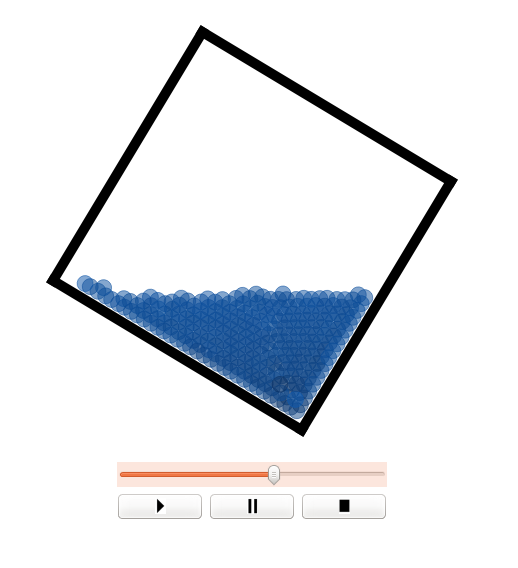
\includegraphics[width=\textwidth]{./rysunki/obrot_stabilny}
 \end{center}
 \caption{Ustabilizowana ciecz}
 \label{fig:obrot_stabilny}
\end{figure}
\end{minipage}\\[0.1cm]

\begin{minipage}{0.5\textwidth}
\begin{figure}[H]
 \begin{center}
  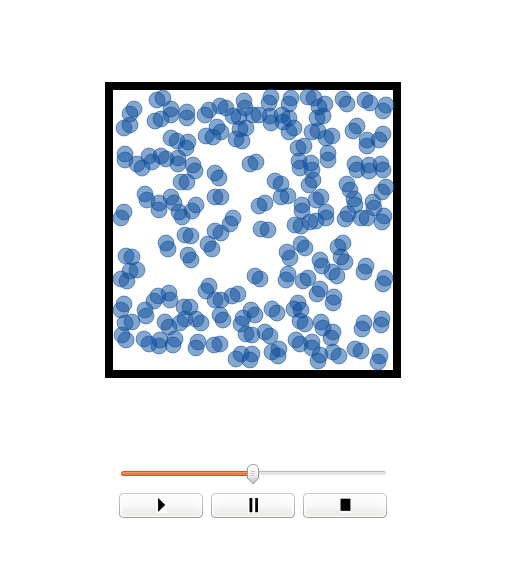
\includegraphics[width=\textwidth]{./rysunki/niewazkosc}
 \end{center}
 \caption{Stan nieważkości}
 \label{fig:niewazkosc}
\end{figure}
\end{minipage}
~
\begin{minipage}{0.5\textwidth}
\begin{figure}[H]
 \begin{center}
  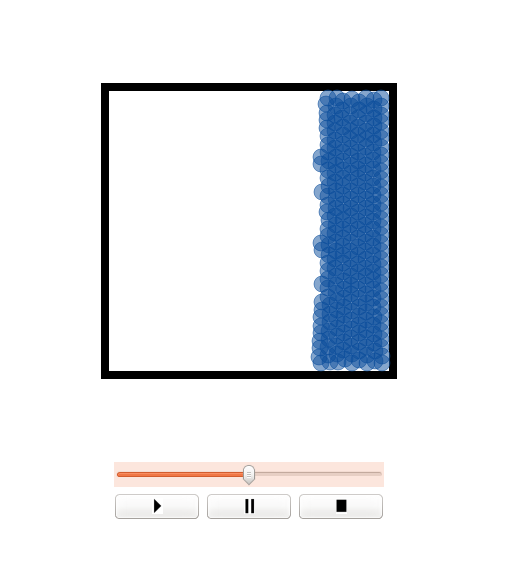
\includegraphics[width=\textwidth]{./rysunki/niewazkosc1}
 \end{center}
 \caption{Stan mikrograwitacji bocznej}
 \label{fig:niewazkosc_stabilny}
\end{figure}
\end{minipage}\\[0.1cm]
